% \begin{wrapfigure}{r}{0.3\textwidth}

%   \centering
%     % \includegraphics[width=0.25\textwidth]{./images/teaser cuted.jpg}
%     % \includegraphics[width=0.15\textwidth]{./images/teaser cuted more.jpg}
%     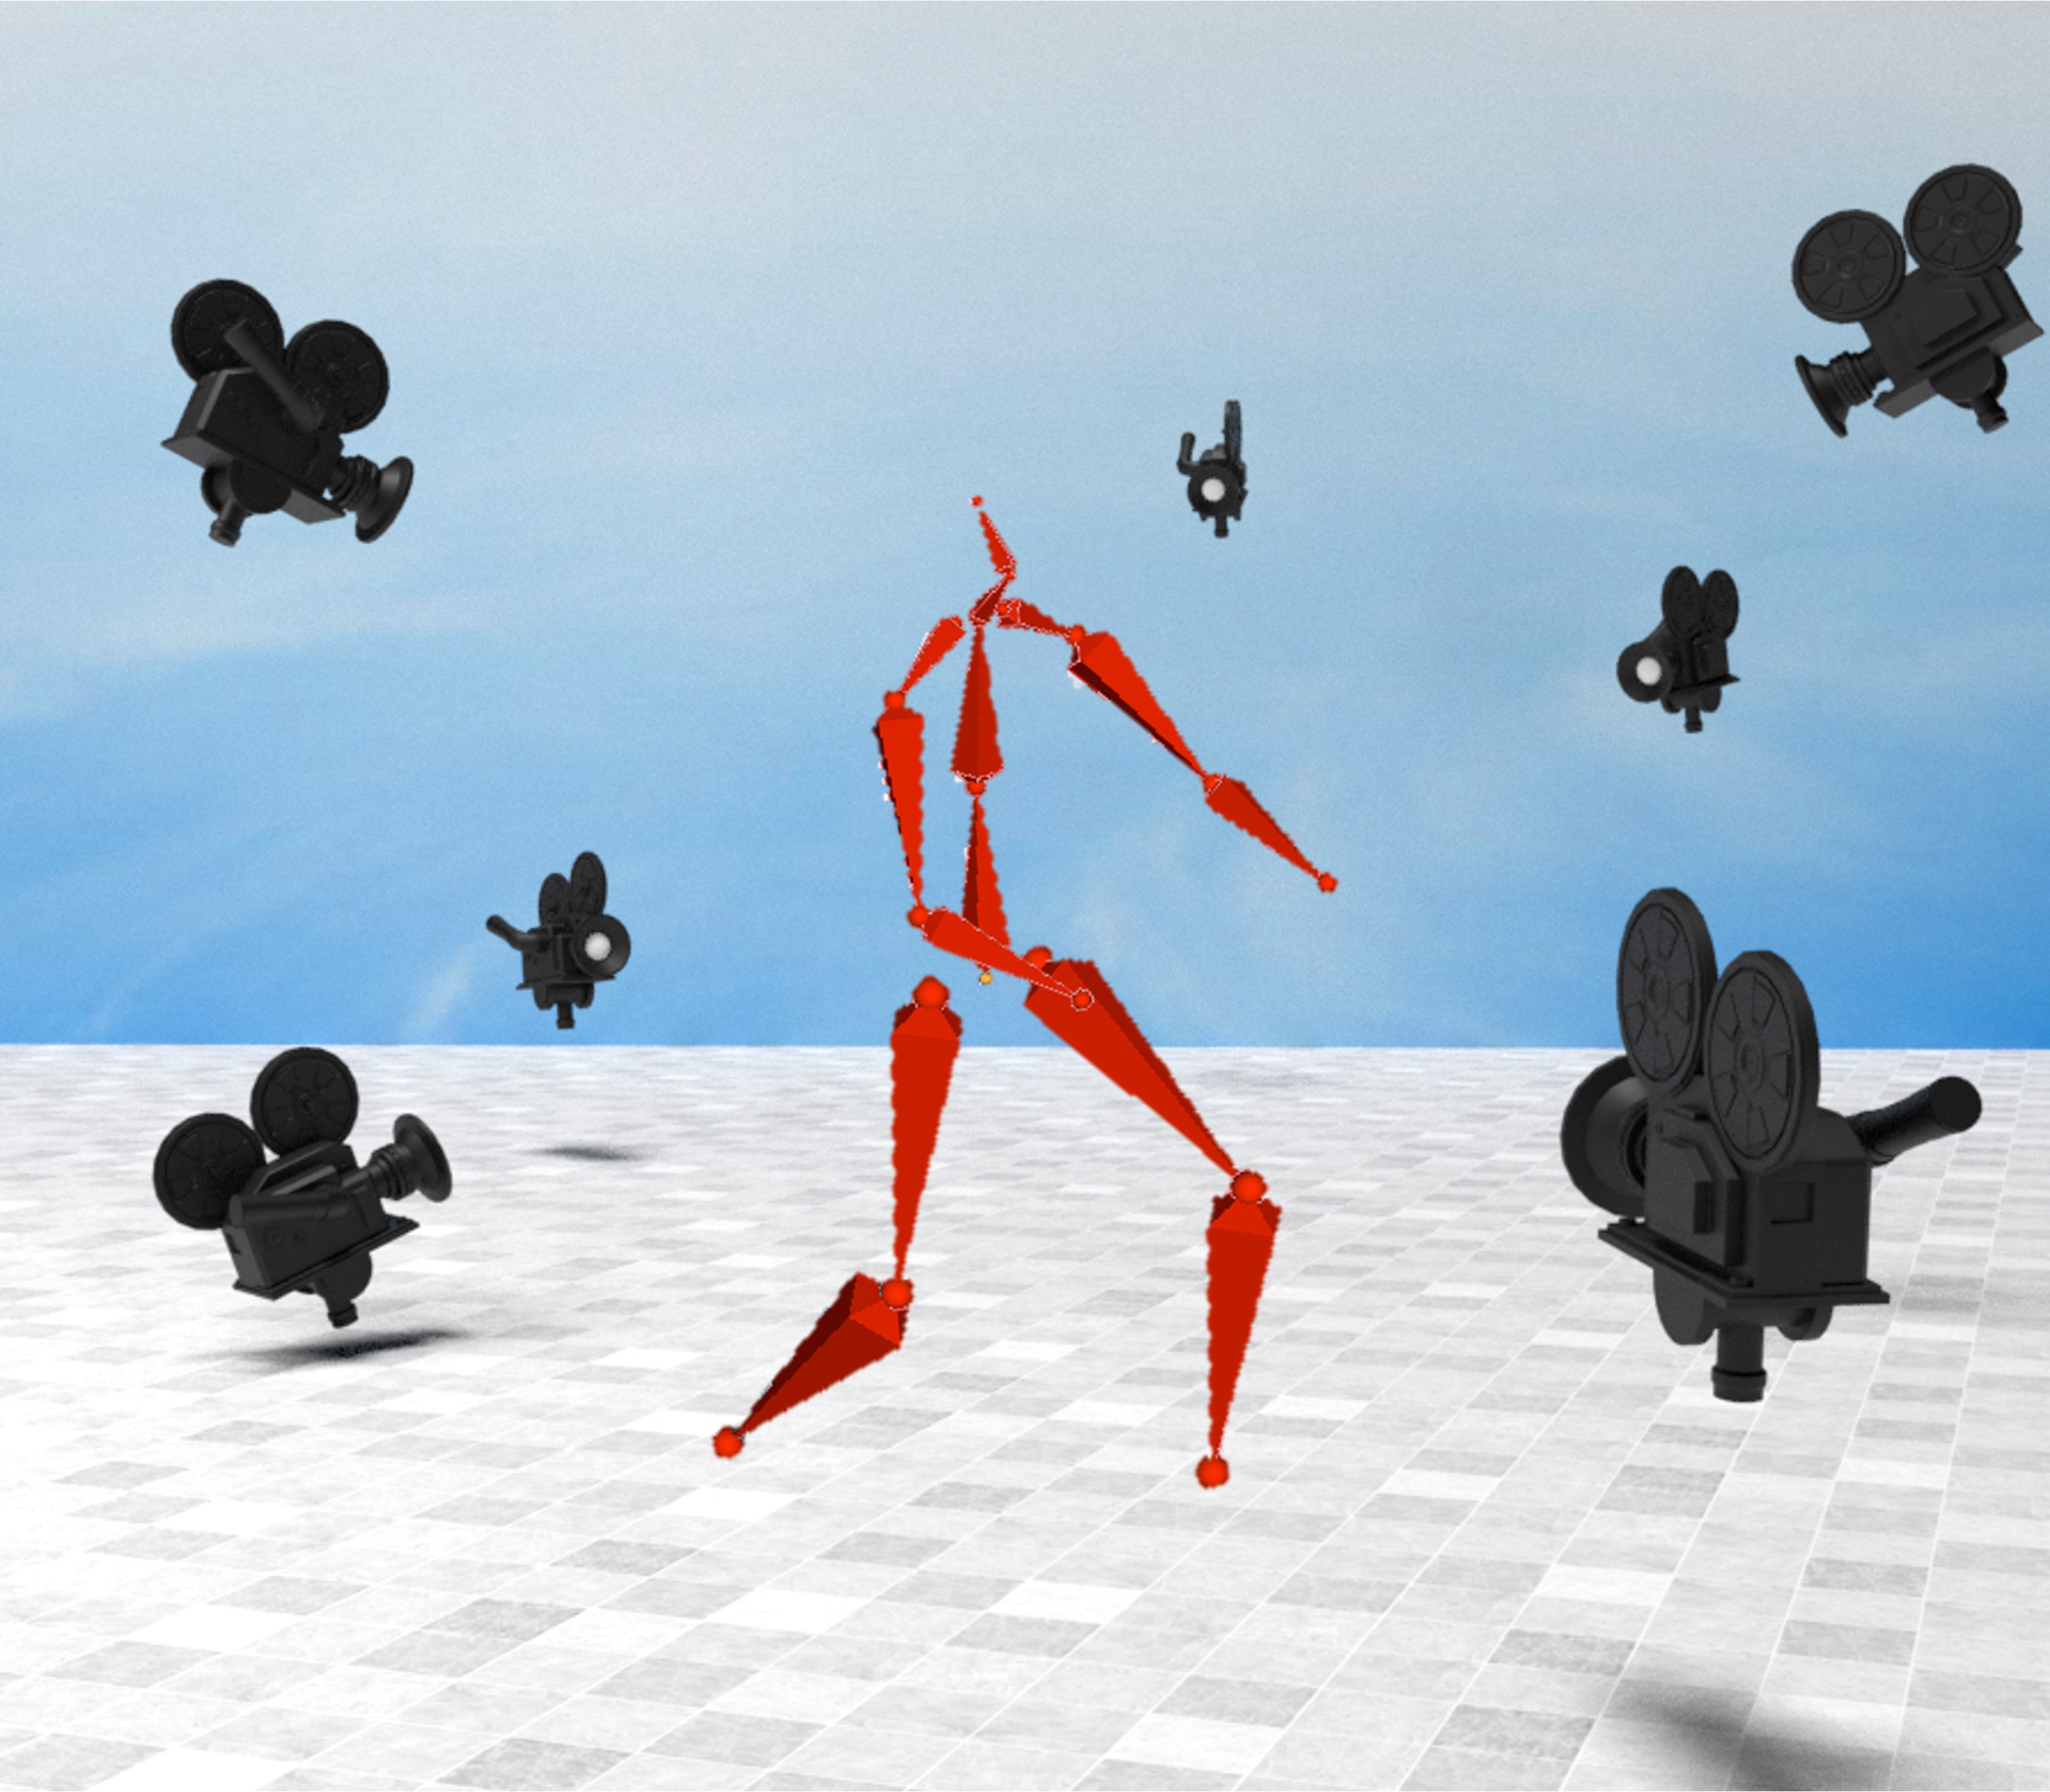
\includegraphics[width=0.3\textwidth]{./images/skeleton_teaser.jpg}
%     % \caption{}
% %   \caption{FLEX reconstructs human motion in environments of multiple cameras, where the camera parameters are unknown.}
% %   \caption{Human motion, captured by multiple cameras.}
%   \label{fig:skeleton_cameras}
% \end{wrapfigure}

\begin{wraptable}{r}{0.48\textwidth}
\setlength{\abovecaptionskip}{-5pt plus 3pt minus 2pt}
\setlength{\belowcaptionskip}{-24pt plus 3pt minus 2pt}

% \begin{table}[h]
\ifeccv
\caption{
%Protocol \#1 
MPJPE 
%error 
on the Ski-PTZ dataset,
measured for methods trained when extrinsic parameters are \emph{not} given. 
%Legend: 
$(\dagger)$ is self/weakly-supervised. 
%$(*)$ is weakly supervised.
}
\fi
\begin{center}
\begin{tabular}{|c|c|}
\hline
\textbf{Method} & \textbf{MPJPE
%(mm) $\downarrow$ 
} \\
\hline
% \hline
% \multicolumn{2}{|l|}{Multi-view methods cam. param. \textbf{ given} } \\
% \hline
% Epipolar Trans.~\cite{he2020epipolar} & 34.2 \\
% TransFusion~\cite{ma2021transfusion} & \textbf{31.6} \\
% \hline
% \hline
% \multicolumn{2}{|l|}{Multi-view methods cam. param. \textbf{ not given} }\\
% \hline
CanonPose~\cite{wandt2020canonpose} ($\dagger$) & 128.1 \\
% \hline
Chen \etal~\cite{chen2021deductive} ($\dagger$) & 99.4 \\
% \hline
Ours & \textbf{65.5} \\
\hline
\end{tabular}
\end{center}

\ifeccv
\else
\caption{Protocol \#1 MPJPE error on the Ski-PTZ dataset,
measured for methods that are trained when extrinsic parameters are \textbf{not} given. 
Legend: $(\dagger)$ is self-supervised. 
$(*)$ is weakly supervised.}
\fi


\label{tab:ski_quantitative}
% \end{table}

\setlength{\abovecaptionskip}{-50pt plus 3pt minus 2pt}
\setlength{\belowcaptionskip}{-0pt plus 3pt minus 2pt}
\caption*{}

\end{wraptable}
